\section{Distribution of Stocks and Portfolios}

\subsection{Individual Stocks}
Investors seek to protect their portfolio, and public equities, now totaling \$51 trillion market value, plays a central role.

We simulated $500,000$ daily returns of an individual stock using the jump-diffusion model of \citet{backus2011disasters}. The model combines a smooth diffusion process, drawn from a normal distribution, with rare discontinuities: jumps whose count follows a shifted geometric distribution and whose size and direction follow a second normal distribution.

Note that stock returns are highly positively skewed. Most stocks perform poorly or modestly on most days, while a small fraction produce outsized gains. Since prices cannot fall below zero, downside is bounded, but upside remains unbounded. This asymmetry shifts the mean return above the median, unlike for a normal distribution where the mean coincides with the median. Studies support this pattern, showing that the median return on individual stocks is often below that of Treasury bills, even though on average, stocks have outperformed bonds by a factor three \citep{bessembinder2018stocks,oh2022cross}.

The parameters for this return simulation reflected the above (see Appendix~\ref{appendix:code}), while emphasizing the skewness of individual stocks. We use a moderate, positive mean return to indicate the long-run equity premium ($\mu = 0.04$), while incorporating a realistic range of fluctuations with the baseline volatility ($\sigma = 0.0324$). The dynamics that dictate variance are $\omega = 0.33$ (jump intensity) $, \theta = 0.12$ (mean jump size) $, \delta = 0.0064$ (volatility of jumps). The resulting distribution in \autoref{fig:fig3} exhibits a skewness of roughly $3$ and kurtosis of $19.8$. 


\begin{figure}[h]
    \centering
    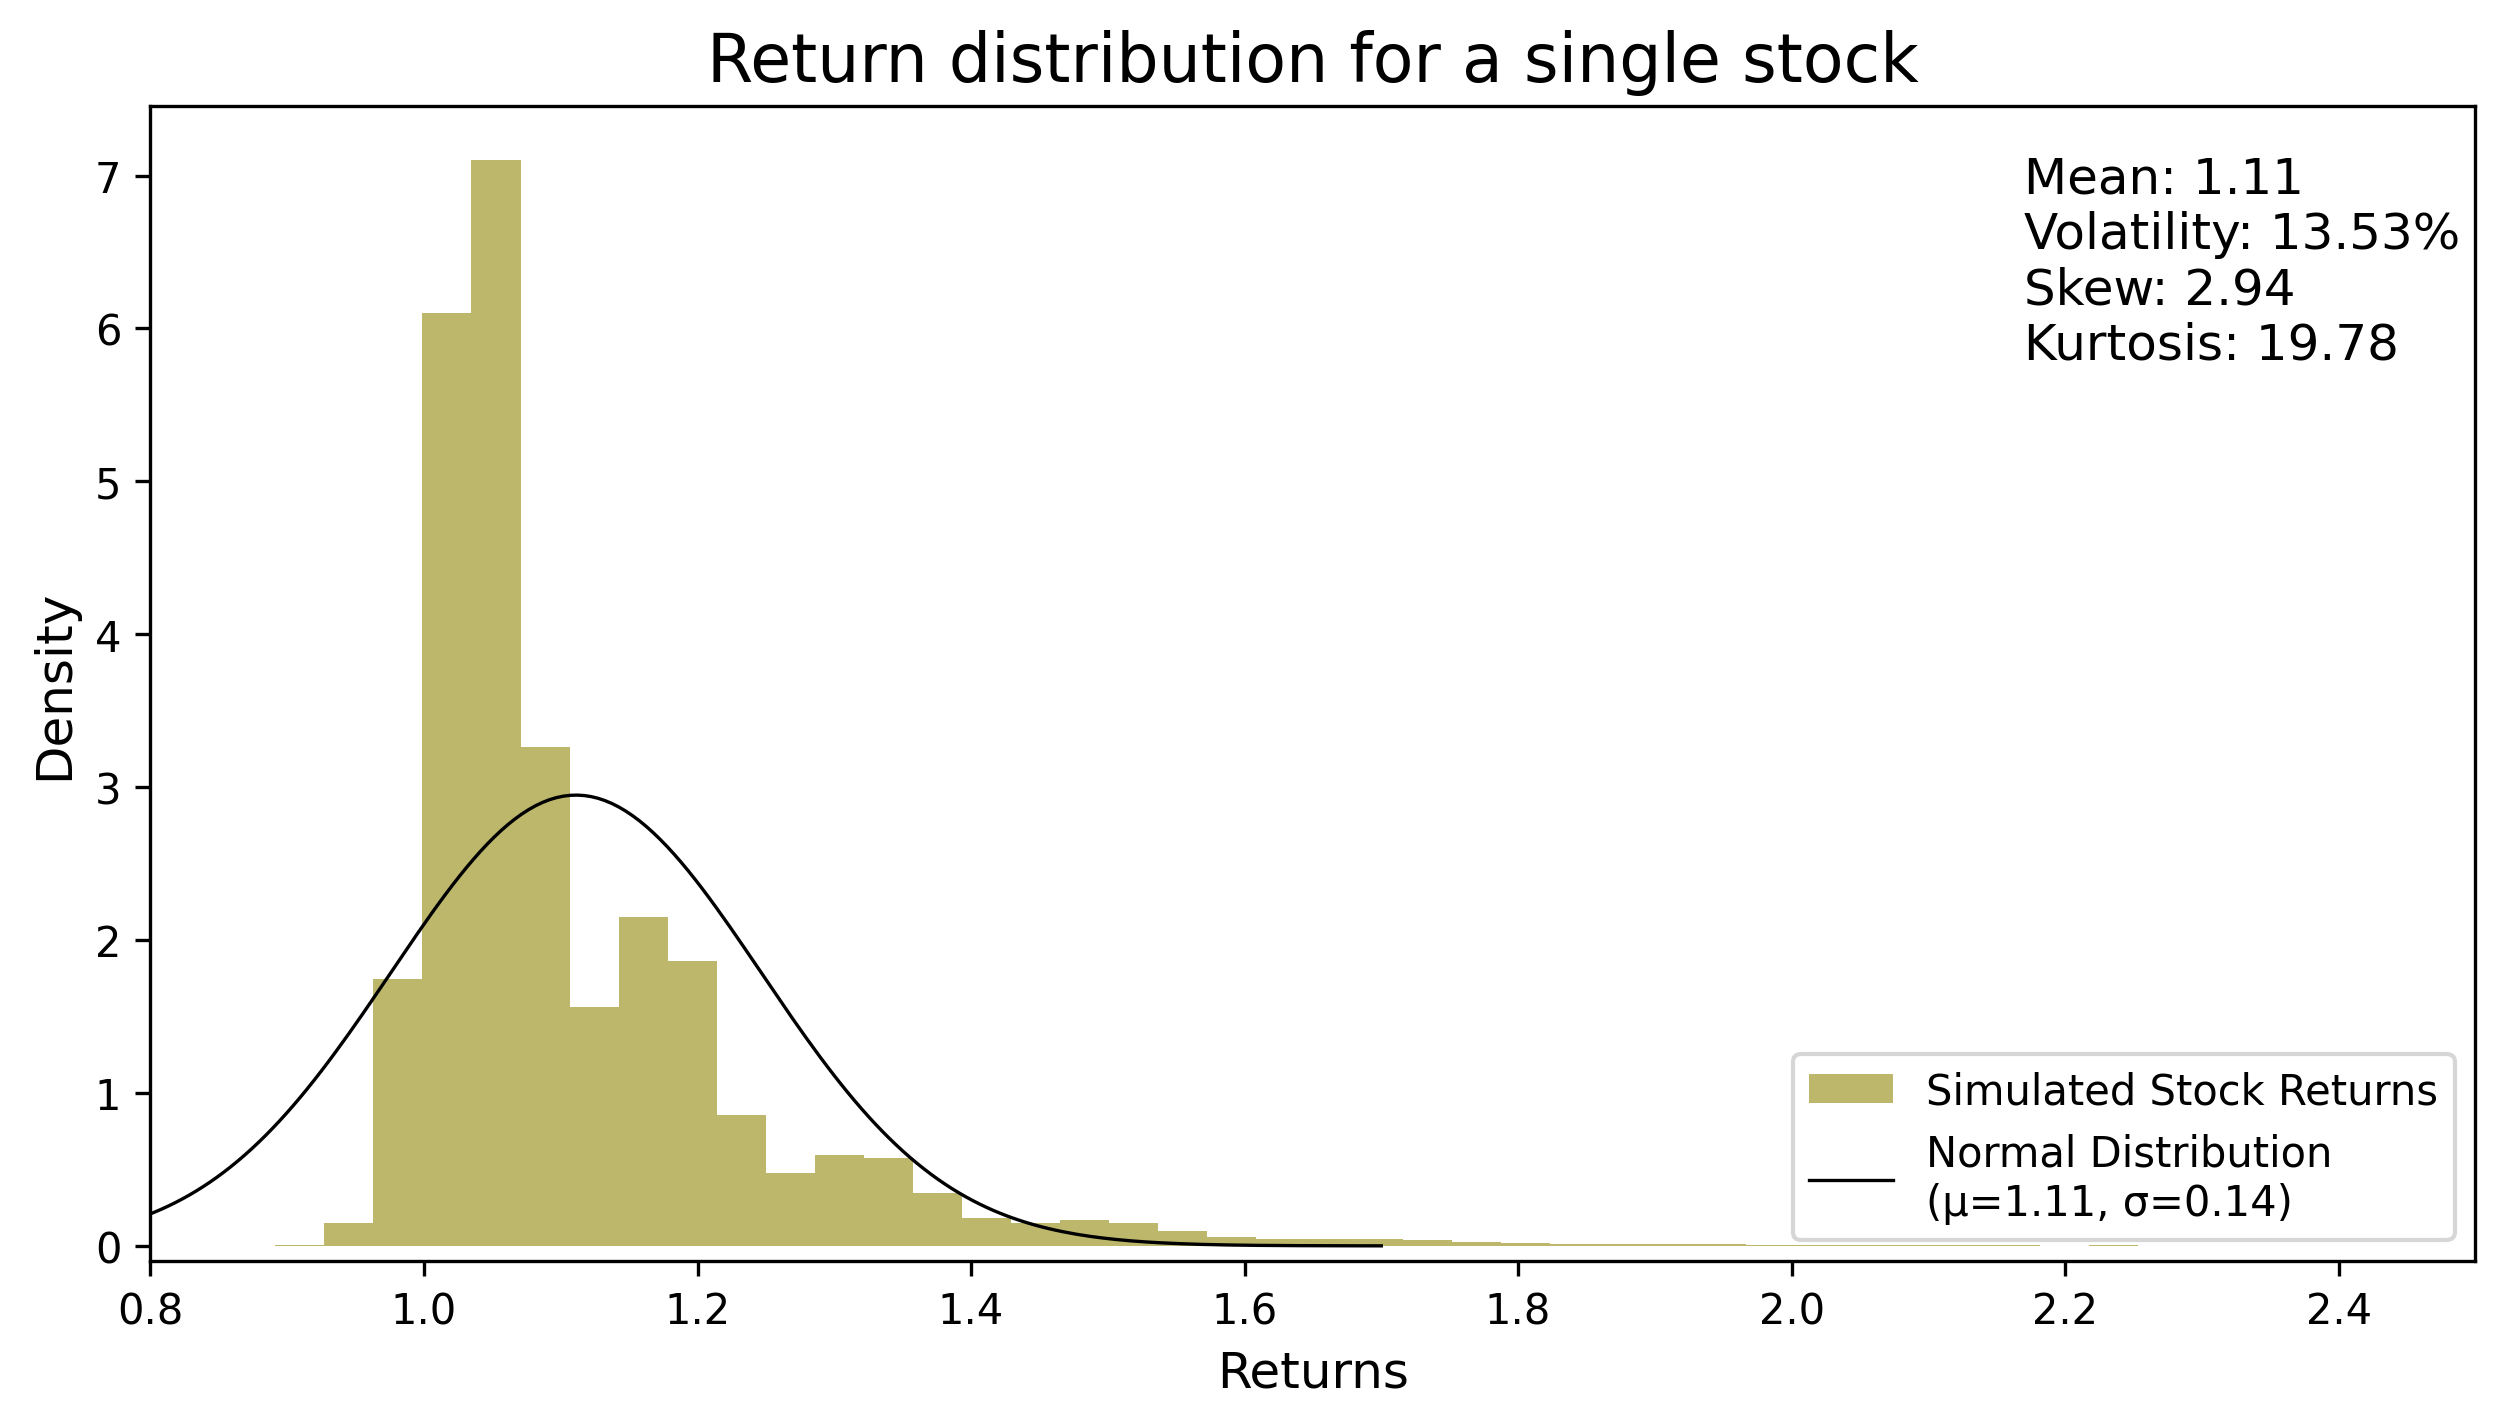
\includegraphics[width=0.75\textwidth]{fig3.png}
    \caption{Simulated return distribution for a single stock, showing strong positive skew and fat tails}
    \label{fig:fig3}
\end{figure}

The positive skew translates into the very long right tail in the distribution. Real stocks echo this pattern. Consider a company developing a new product (such as a new gene therapy treatment). The product may face a high probability of failure, yet if it succeeds, the benefits will be large. This payoff structure creates the right-skewed distribution of daily returns that appears in many small-cap biotech firms, like Sarepta Therapeutics, which exhibits a skewness of $8.49$ (\autoref{fig:fig4}). Most days produce modest or negative returns, but occasional breakthroughs, regulatory approvals, or acquisitions generate outsized gains. 
Note the extraordinarily high kurtosis in \autoref{fig:fig4}, measured at 248. This extreme value arises from a handful of outlier days with gross returns much higher than the mean (approximately $2.00, 1.46,$ and $1.03$). Such rare but very large deviations inflate the tails of the distribution, driving kurtosis upward.

Similarly, the high kurtosis in \autoref{fig:fig3} indicates that extreme events occur in individual stock returns more often than a normal model would suggest. Even a large, diversified company such as Apple displays high kurtosis (\autoref{fig:fig5}) in its daily return distribution (despite relatively low skew) because its returns still experience fat-tailed shocks. 

\begin{figure}[h]
    \centering
    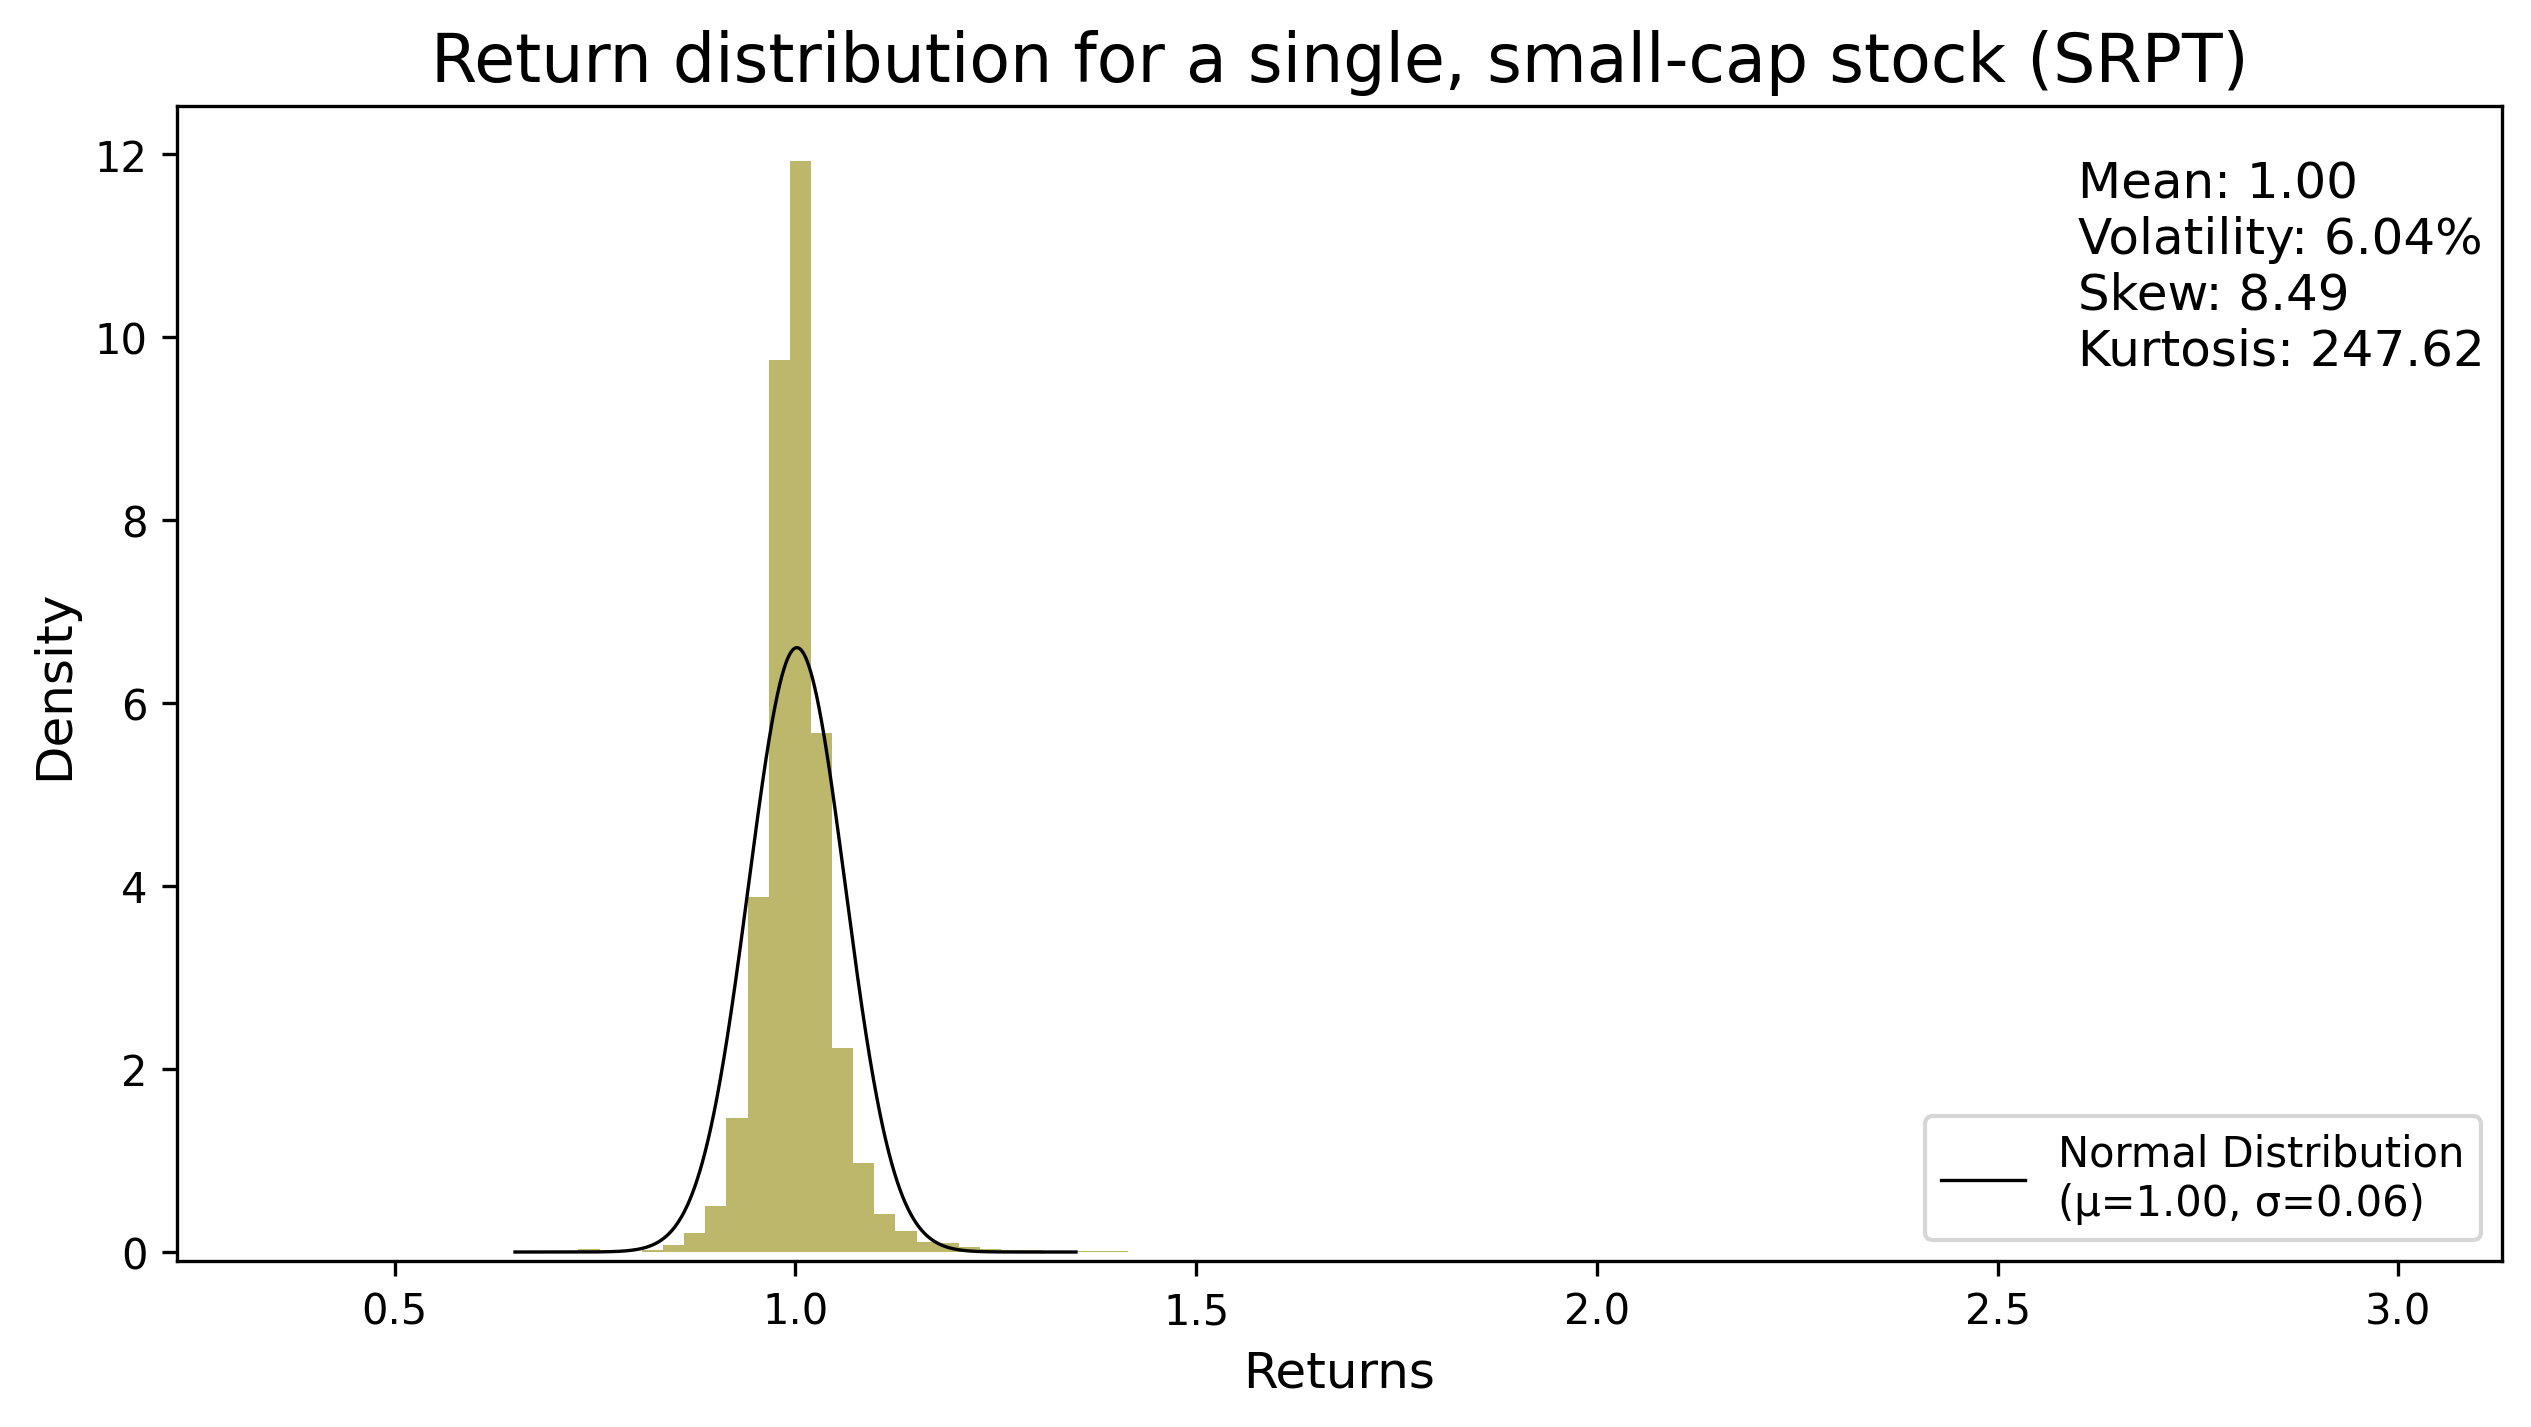
\includegraphics[width=0.75\textwidth]{fig4.png}
    \caption{Empirical return distribution of Sarepta Therapeutics}
    \label{fig:fig4}
\end{figure}

\begin{figure}[h]
    \centering
    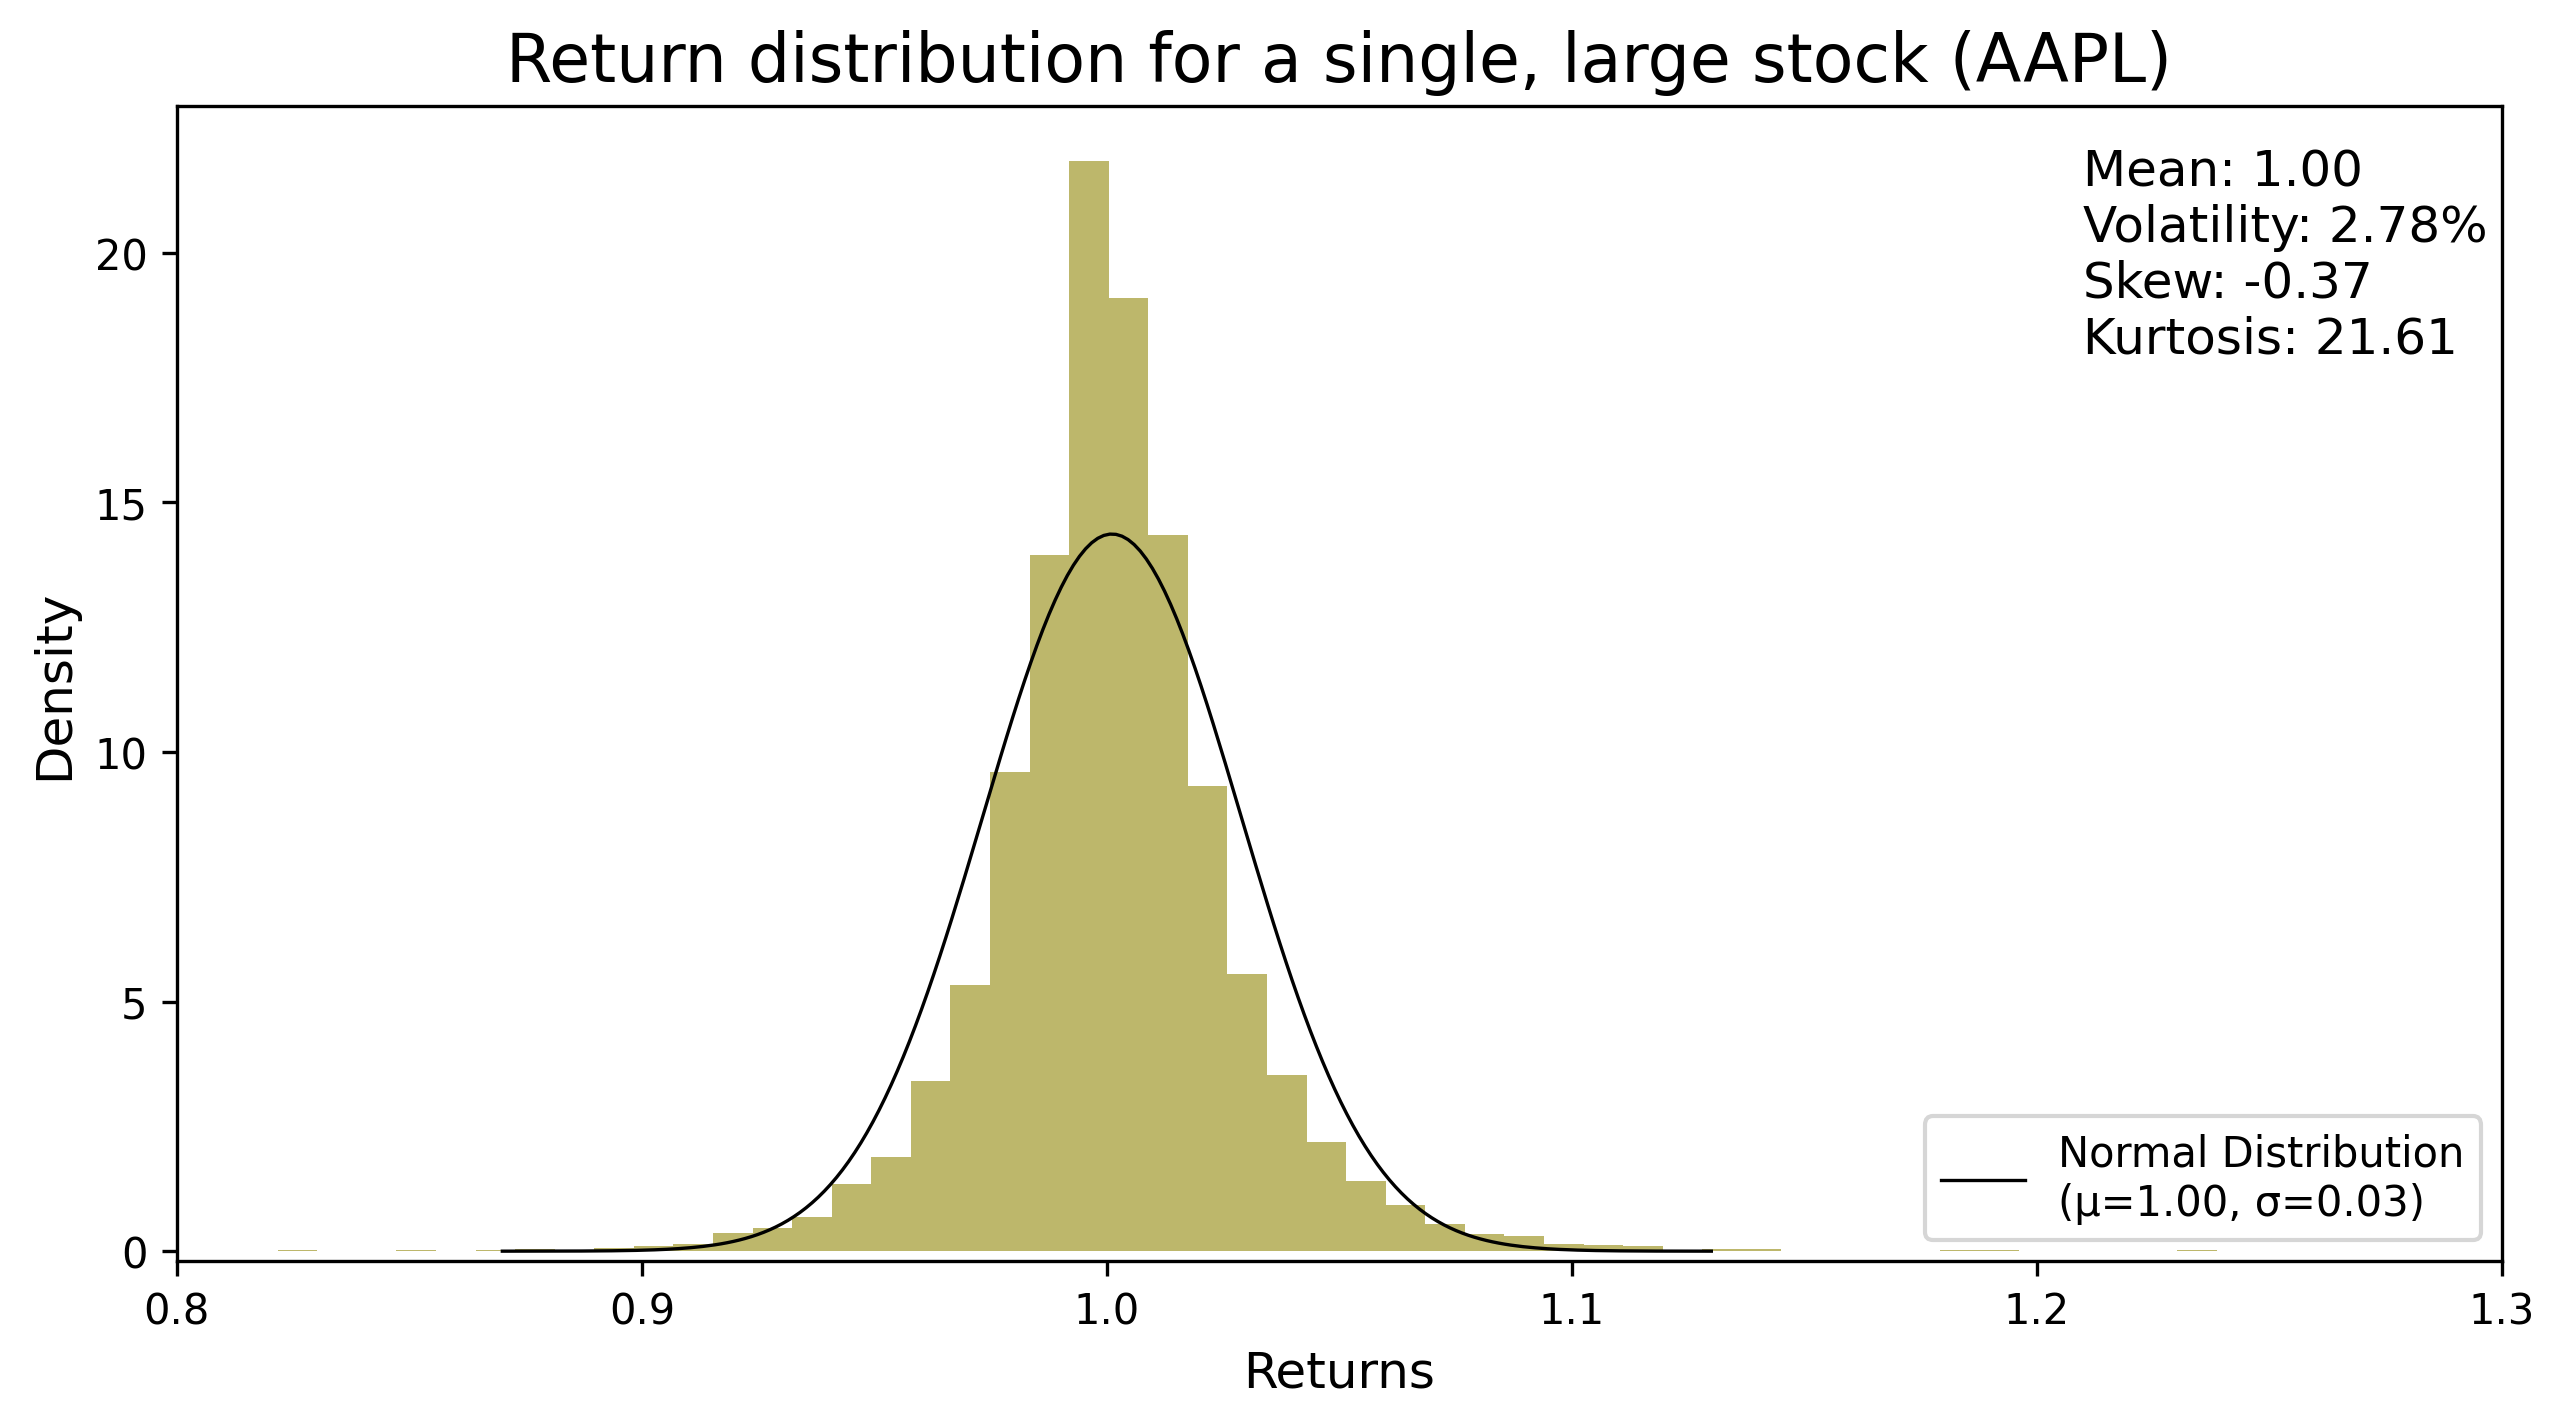
\includegraphics[width=0.75\textwidth]{fig5.png}
    \caption{Return distribution of Apple}
    \label{fig:fig5}
\end{figure}

These return distributions are risky, in that they are not well-captured by variance alone. High skew and fat tails imply that mean-variance analysis misses much of the story.

\subsection{Portfolio Returns}
The issue with individual stocks is the wild returns. However, the central limit theorem predicts that summing many independent variables results in a normal distribution. Furthermore, the law of large numbers tells us that the variance should approach zero.  

We construct a diversified portfolio by averaging 100 independent and identically distributed stocks from the model used in \autoref{fig:fig3}. Each simulated portfolio return is the mean of 100 stocks at each date $t$ (see Appendix~\ref{appendix:code}). The resulting distribution of daily returns is shown in \autoref{fig:fig6}.

\begin{figure}[h]
    \centering
    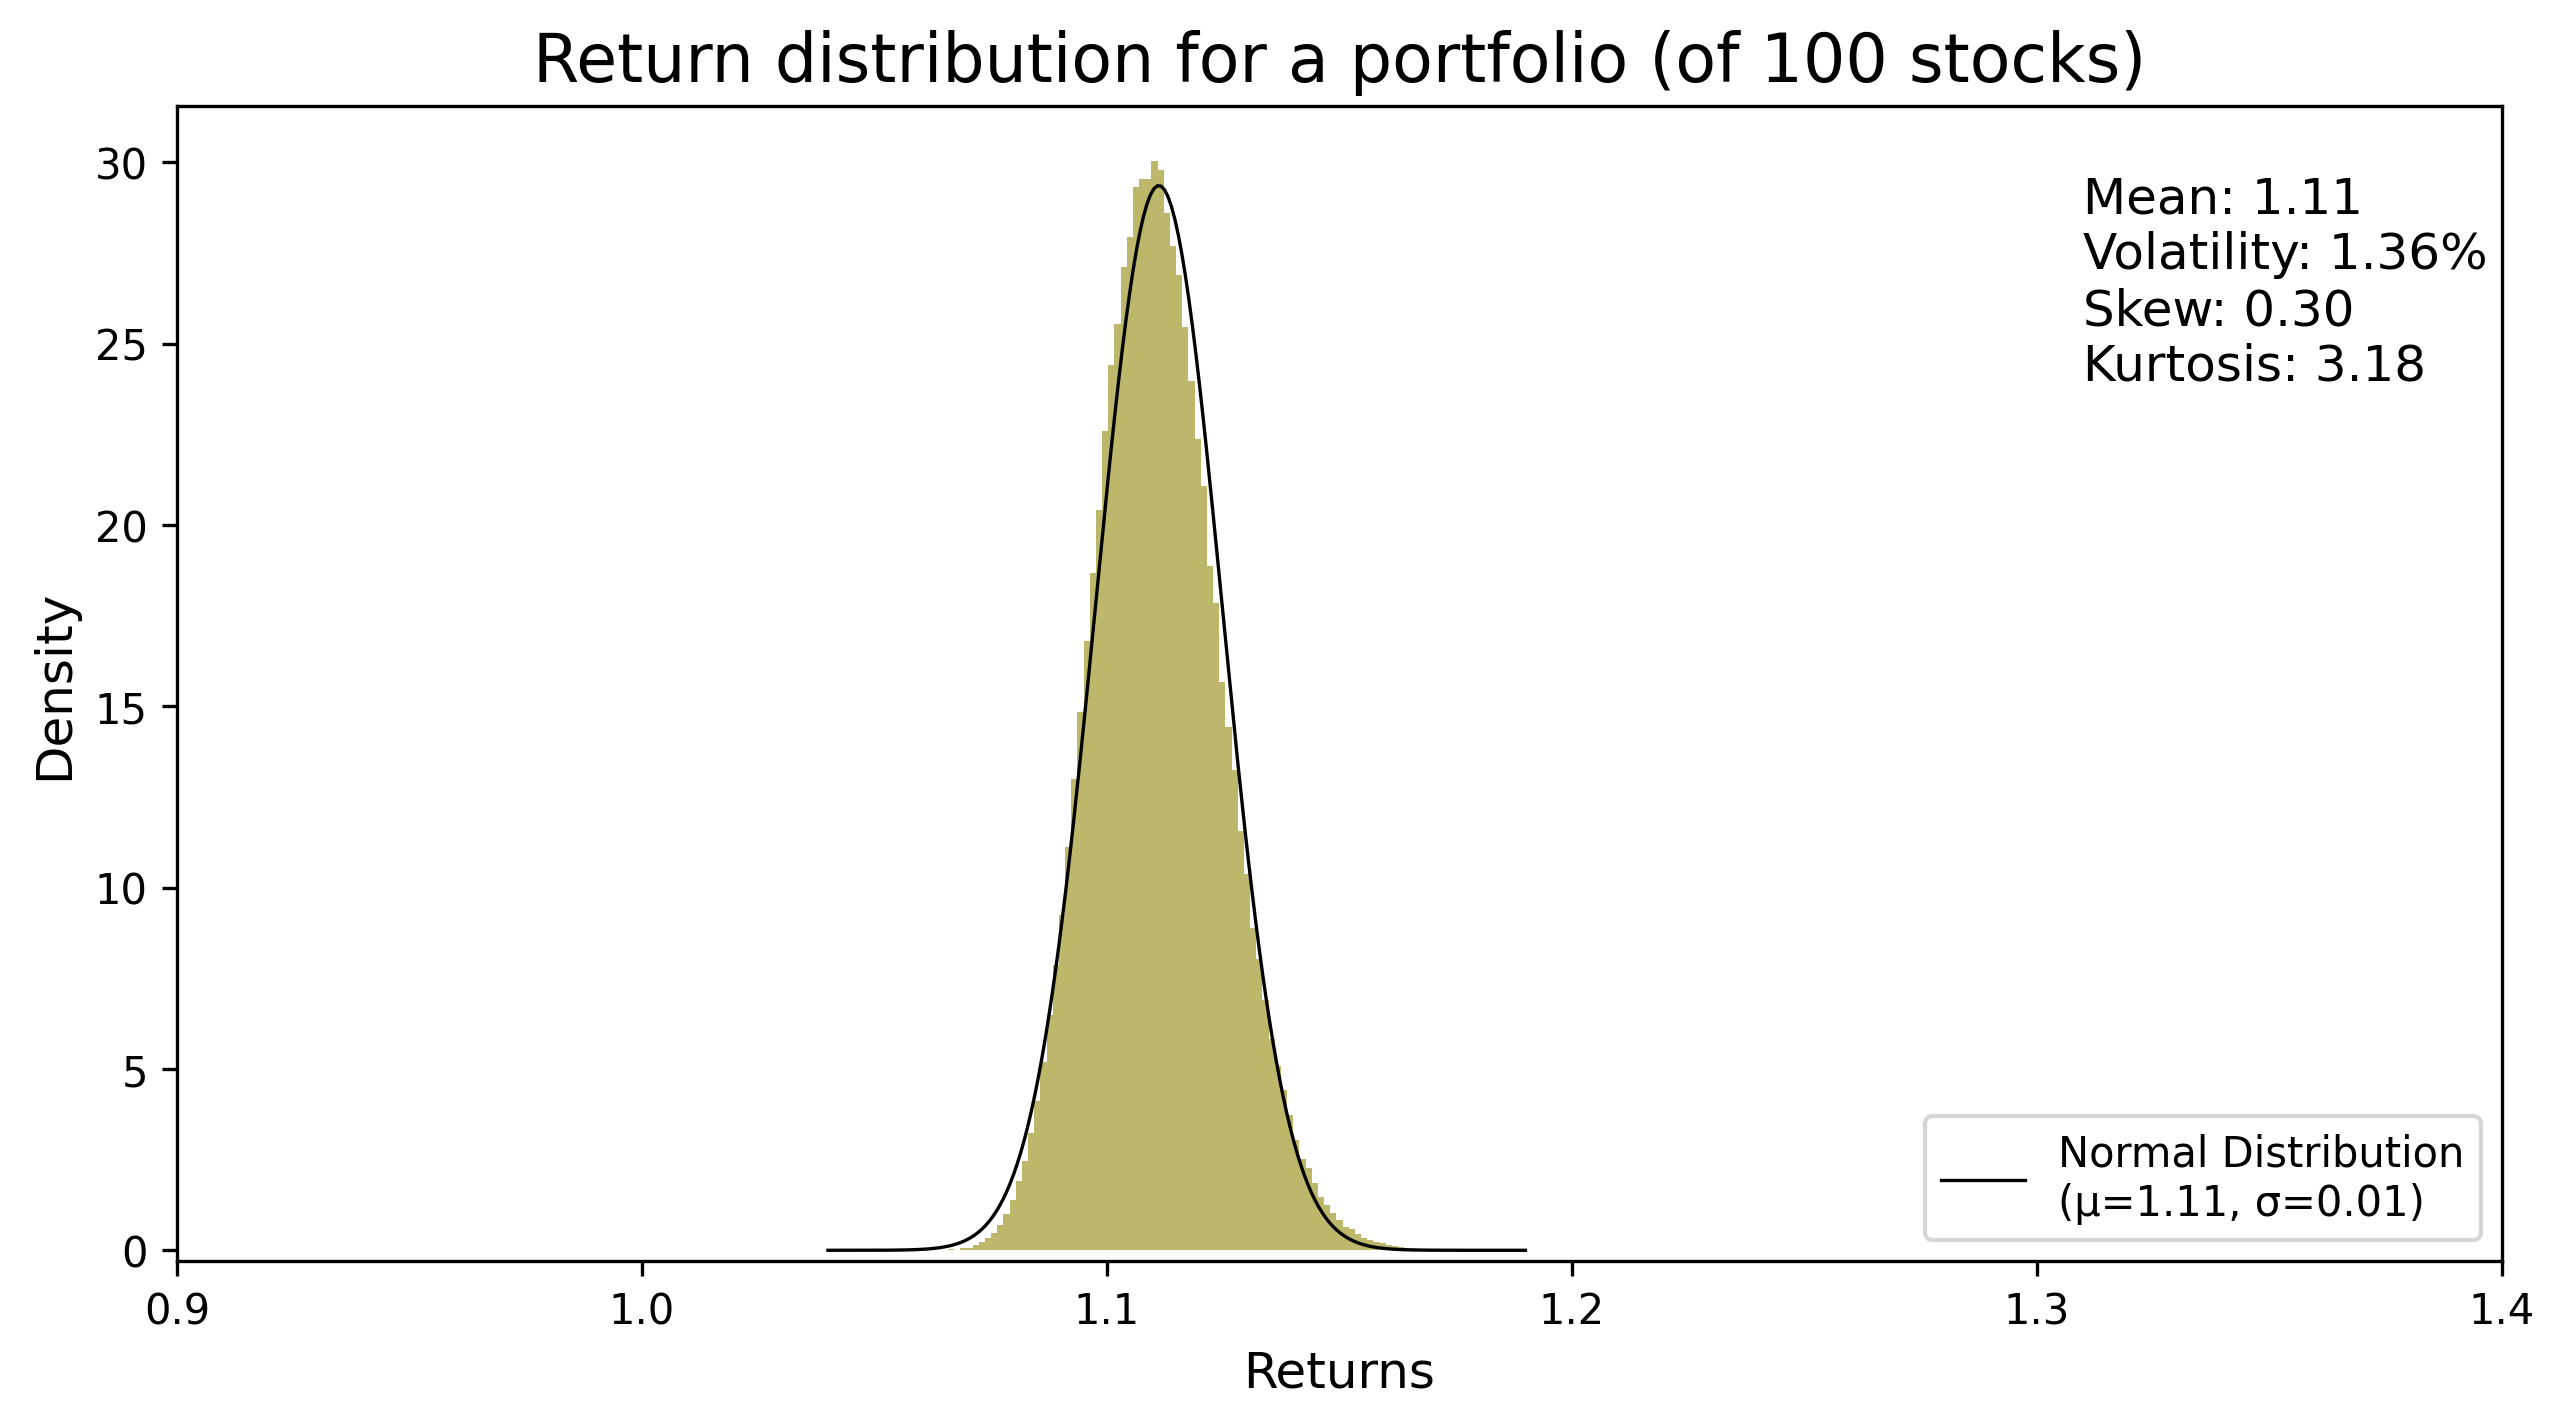
\includegraphics[width=0.75\textwidth]{fig6.png}
    \caption{Simulated portfolio daily return distribution from averaging 100 stock simulations}
    \label{fig:fig6}
\end{figure}

The portfolio shows low skew ($= 0.30$) and near-normal kurtosis ($= 3.18$). Thus, diversification removes much of the \say{unexpectedness} in individual stock returns. The fat right tails of some firms are offset by the poor returns of others, resulting in a thinner-tailed, symmetric return profile with a lower variance.

However, diversification does not eliminate risk; it transferred from undiversified investors to a wide pool of capital providers. Capital providers must trust firm managers to deploy funds responsibly. But once capital is raised, managers may bear little downside and capture most of the upside. They may shrink, take excessive risks, or divert resources toward perks. The very act of pooling capital introduces moral hazard. For diversification to work, agency problems must be solved.